\documentclass[10pt,a4paper]{article}
\usepackage[utf8]{inputenc} % para poder usar tildes en archivos UTF-8
\usepackage[spanish]{babel} % para que comandos como \today den el resultado en castellano
\usepackage{fullpage} %small margins
\usepackage[parfill]{parskip} %genera saltos entre parrafos
\usepackage{color}
\definecolor{gray}{gray}{0.35}
\usepackage{listings}
\usepackage{enumitem}
\usepackage{amsmath} %big brackets
\lstset{
    numbers=left,
    breaklines=true,
    tabsize=2,
    basicstyle=\ttfamily\color{gray},
}
\setlength{\parindent}{8pt}
\usepackage{mathtools}
\usepackage[margin=50pt]{geometry}
\usepackage{amsfonts}
\usepackage{flafter}
\usepackage{multicol}

\begin{document}

\section{Heurística constructiva golosa}
\subsection{Desarrollo}
\subsubsection{Ideas preliminares}

Partiremos de la siguiente premisa: el enunciado del problema nos presenta un grafo con nodos y aristas con peso que iniciden sobre los mismos. Podemos de esta forma pensar en ``nodos con peso'': el peso de un nodo es el peso de las aristas que inciden sobre él.


\subsubsection{Explicación del algoritmo}

En primer lugar, definiremos la noción de \textit{peso\_intrapartición} ya que sera relevante a lo largo del algoritmo. 
Llamaremos \textit{peso\_intrapartición} de un nodo a la suma de los pesos de las aristas que inciden sobre un él en un partición de nodos dados.
A continuación, presentamos un pseudocódigo de la función que calcula el peso\_intrapartición de un nodo en una partión, según las aristas de un grafo dado.\\
Si la partición es vacía, es decir, si el nodo va a insertarse en un subconjunto solo, como no va a haber aristas que incidan sobre él, su peso\_intrapartición será 0.\\
Caso contrario, se iterará sobre todos los nodos presentes en la partición y para cada uno, se buscará el peso de la arista entre éste y el nodo que se quiere averiguar el peso\_intrapartición y se irá sumando ese resultado. A terminar de iterar el conjunto, se tendrá el peso\_intrpartición del nodo.

Sea conjunto = set(int)

\begin{lstlisting}
int peso_intraparticion(int i, grafo g, conjunto particion){
	if(particion.empty){
		return 0
	} else{
		sumaPesos <- 0
		for(nodo in particion){
			sumaPesos += grafo[i][nodo]
		}
	}
	return sumaPesos
}
\end{lstlisting}

A continuación, el algoritmo constructivo goloso.\\
Describiremos la solución implementada, dividiéndola en dos etapas.

\bigskip
\begin{enumerate}
\item


\textbf{Preparación de los datos en distintas estructuras:} 

Recepción del input y su posterior implementación como la matriz de adyacencias del grafo que se pasó como parámetro. Utilizamos una matriz de enteros, en el que en cada posición i:j guardamos el peso de la arista que incide sobre los nodos i y j. En caso de que dichos nodos no sean adyacentes, consideramos peso 0.

A continuación, creamos las estructuras necesarias para obtener la solución y devolver el resultado de la instancia. En el siguiente fragmento de pseodocódigo mostramos las operaciones realizadas.\\\\

Sea k = cantidad de particiones pasadas como input.\\
Sea n = cantidad de nodos pasados como input.\\
Sea nodoConPeso un struct en el que representamos un nodo según su id y su peso\_intrapartición en un conjunto determinado. Este struct cuenta con la operación de comparaciónPorPeso que justamente, compara dos nodoConPeso por su peso.\\
Sea g = la matriz de adyacencia formada a partir del grafo pasado como input, según los nodos y las aristas (con su respectivo peso) incidentes a cada uno de los nodos.\\
Sea conjunto = vector(set(int)).\\
\newpage

\begin{lstlisting}[mathescape]
particiones <- vector(conjunto) de k elementos
conjuntoNodos <- conjunto
for(nodo in n){
	inserto nodo en conjuntoNodos
}

pesos <- vector(nodoConPeso) de n elementos
for(nodo in n){
	pesos[nodo] <- nodoConPeso(nodo, peso_intraparticion(nodo, g, conjuntoNodos))
}

ordenar el vector pesos de manera creciente usando ComparacionPorPeso.
\end{lstlisting}


\textit{Particiones} representa los k conjuntos de nodos en los que podemos subdividir a los nodos. Este dato fue pasado como parámetro del problema en el input.

Insertamos en \textit{conjuntoNodos} los n nodos, o más bien, el entero que los representa para poder usar luego este conjunto para calcular el peso\_intrapartición de los nodos cuando se encuentran todos en un mismo conjunto, es decir, como se encuentran en el grafo originalmente.

Creamos un vector de n posiciones, \textit{pesos} en el que almacenaremos los  los n nodosConPeso, utilizando para cada nodo el peso\_intrapartición que del nodo en el \textit{conjuntoNodos}. Por último, lo ordenamos. De esta forma, los nodos quedan ordenados en el vector \textit{pesos} del más \"pesado\", es decir, aquel que su peso\_intrapartición era mayor en \textit{conjuntoNodos}.\\

\item \textbf{Alogritmo greedy:}
En esta etapa trabajamos sobre el vector \textit{pesos}. Tomaremos cada uno de los nodos guardados en él (como lo ordenamos en el paso anterior, iremos tomando desde los nodos más \"pesados\" hasta los más \"livianos\").\\
La idea subyacente será, para cada uno de los nodos tomados en orden, encontrar cuál es el conjunto del vector \textit{particiones})en el cuál el nodo tiene peso\_intrapartición mínimo.\\
Entonces, por cada uno de los nodos de \textit{pesos}, tomamos como su menorPeso (inicial) al peso\_intrapartición de ese nodo en \textit{conjuntoNodos}.\\
Luego, para cada uno de los k subconjuntos de \textit{particiones} chequeamos si el peso del nodo en la partición que se esta chequeando es menor o igual al menorPeso guardado hasta el momento. Si lo es, actualizamos el menorPeso y guardamos el subconjunto en el que fue encontrado.\\
Al terminar de chequear en los k conjuntos, tenemos el conjunto en el que un nodo alcanza su peso\_intrapartición mínimo, entonces, lo sacamos de \textit{conjuntoNodos} y lo ponemos en el nuevo subconjunto. Nótese que como al comenzar el algoritmo se calcula el menorPeso del nodo en  \textit{conjuntoNodos}, tras sacar un nodo de éste, se calcula el peso del siguiente nodo en un conjunto \textbf{sin} el nodo que fue sacado en una iteración previa.\\
\end{enumerate}

\begin{lstlisting}[mathescape]
for nodo in pesos{
	menorPeso <- peso_intraparticion(nodo, g, conjuntoNodos)
	for(l in k){
		pesoEnL <- peso_intraparticion(nodo, g, particiones[l])
		if(pesoEnL <= menorPeso){
			menorPeso <- pesoEnL
			particionElegida <- l
		}
	}
	conjuntoNodos.erase(nodo)
	particiones[particionElegida].insert(nodo)
}
\end{lstlisting}


Al terminar las n iteraciones, en el vector \textit{particiones} tenemos todos los nodos que se pasaron como input pero colocados en el conjunto en el cuál su peso\_intrapartición era el menor (en el momento en que se evaluó ese nodo) y por lo tanto, la suma de los pesos\_intrapartición de los nodos de todos los subconjuntos es mínima, lo cuál es una solución al problema.


\newpage
\subsection{Complejidad}

Para el análisis de complejidad, dividiremos nuevamente al problema en secciones como en el inciso anterior. Para comodidad del lector y facilidad de lectura, transcribiremos los fragmentos de pseudocódigo pertinentes a la demostración.
Como en el apartado anterior, describimos algunos renombres:


Sea k = cantidad de particiones pasadas como input.\\
Sea n = cantidad de nodos pasados como input.\\
Sea nodoConPeso un struct en el que representamos un nodo según su id y su peso\_intrapartición en un conjunto determinado. Este struct cuenta con la operación de comparaciónPorPeso que justamente, compara dos nodoConPeso por su peso.\\
Sea g = la matriz de adyacencia formada a partir del grafo pasado como input, según los nodos y las aristas (con su respectivo peso) incidentes a cada uno de los nodos.\\
Sea conjunto = vector(set(int)).\\


\textbf{\underline{Sección I-Auxiliar:} Análisis de la función peso\_intrapartición}

\begin{lstlisting}
int peso_intraparticion(int i, grafo g, conjunto particion){
	if(particion.empty){
		return 0
	} else{
		sumaPesos <- 0
		for(nodo in particion){
			sumaPesos += grafo[i][nodo]
		}
	}
	return sumaPesos
}
\end{lstlisting}

Para esta sección tenemos, en la segunda línea, el chequeo de si un set de enteros es vacío. Esto tiene complejidad $O(1)$ según la documentación de C++.
Luego, en la línea 6 iteramos sobre un set de enteros lo cual tiene una complejidad lineal sobre la cantidad de elementos del set (ya que el set de la librería de C++ está implementado sobre un ABB), por lo que n veces realizamos una asignación en una variable.\\
Para representar al grafo utilizamos un vector de vectores de enteros. El vector tiene n elementos, y cada vector también (ya que estamos representando al grafo en una matriz de adyacencias). De esta forma, la asignación mencionada anteriormente tiene complejidad constante, ya que es tomar el elemento ij en la matriz.\\
Por lo tanto, en esta sección tenemos la siguiente complejidad temporal:\\
$O(1)$ (Por chequear si el set es vacío y devolver 0 si ese es el caso) y $n*(O(1))$ en el caso de que el set no sea vacío y haya que iterar el set de nodos y asignar en la variable el valor de la matriz.\\
Finalmente, la complejidad de obtener el peso\_intrapartición de un nodo termina siendo $O(n)$.


\textbf{\underline{Sección II:} Recepción y preparación del input} 

\begin{lstlisting}[mathescape]

particiones <- vector(conjunto) de k elementos
conjuntoNodos <- conjunto
for(nodo in n){
	inserto nodo en conjuntoNodos
}

pesos <- vector(nodoConPeso) de n elementos
for(nodo in n){
	pesos[nodo] <- nodoConPeso(nodo, peso_intraparticion(nodo, g, conjuntoNodos))
}

ordenar el vector pesos de manera creciente usando ComparacionPorPeso.
\end{lstlisting}


En esta sección tenemos, en la primera línea crear un vector de conjuntos. El vector tiene k elementos, y como crear un set vacío tiene complejidad constante, la complejidad de la creación del vector \textit{particiones} es lineal en k.\\
En la línea 2, tenemos la creación de un conjunto en el que, en las siguientes líneas insertaremos los enteros que representan a los n nodos pasados como parámetros. La creación del conjunto, como mencionamos anteriormente, es constante. La inserción es logarítimica en la cantidad de elementos del conjunto, por lo que la complejidad termina resultando $O(n*log (n))$, ya que en el peor caso, en el conjunto están todos los nodos.

En la línea 7, creamos un vector de nodoConPeso vacío y con n posiciones, y en la línea siguiente, en cada posición del vector creamos un nodoConPeso. Insertar en el vector tiene complejidad constante, ya que como tine n posiciones y no vamos a insertar más de n nodos, el vector no se va a redmiensionar. Sin embargo, la asignación del peso del nodoConPeso tiene la complejidad de calcular el peso\_intrapartición de un nodo en un set de nodos, que en el peor caso puede contenerlos a todos. De esta forma, la complejidad de las líneas 6 y 7 queda $O(n)$ (por la creación del vector de n posiciones) + $n*(O(n))$(por calcular n veces la complejidad del peso\_intrapartición de un nodo, que en el peor caso cuesta $O(n)$). Entonces, la complejidad de estas líneas es de O($n^2$) en peor caso.\\
Finalmente, en la línea 12 realizamos el ordenamiento, utilizando el sort de la librería stl de C++, cuya complejidad es $O(n log n)$, siendo n la cantidad de elementos a ordenar(en este caso, son la cantidad de nodos). Como función de comparación usamos la comparaciónPorPeso que compara el peso de dos nodoConPeso, y cuya complejidad es constante.\\
Entonces, para esta sección, la complejidad temporal es:\\
$k + O(n*log(n))+O(n)+ O(n^2)+O(n*log(n)) = k + 2*O(n*log(n)) + O(n) + O(n^2) = k +  O(n^2)$\\

\textbf{\underline{Sección 3:} Algoritmo greedy}

\begin{lstlisting}[mathescape]
for nodo in pesos{
	menorPeso <- peso_intraparticion(nodo, g, conjuntoNodos)
	for(l in k){
		pesoEnL <- peso_intraparticion(nodo, g, particiones[l])
		if(pesoEnL <= menorPeso){
			menorPeso <- pesoEnL
			particionElegida <- l
		}
	}
	conjuntoNodos.erase(nodo)
	particiones[particionElegida].insert(nodo)
}
\end{lstlisting}

Para la última sección del algoritmo, tenemos, en la primer línea, la iteración sobre un vector de n elementos.\\
En la línea 2, tenemos la asignación en una variable del peso\_intrapartición de un nodo, lo cual como vimos en la Sección I tiene complejidad lineal sobre la cantidad de nodos.\\
Luego, k veces obtener el peso\_intrapartición de un nodo en una partición, lo que en peor caso tiene complejidad lineal, como mencionamos ya previamente. Después de esta asignación, relizamos en las líneas subsiguientes (5, 6, 7) operaciones de complejidad constante, tales como comparaciones entre enteros y asignación en variables. Entonces entre las líneas 4 y 7 tenemos una complejidad asintótica de $O(n) + 3*O(1) = O(n)$.\\
Por último realizamos en las últimas dos líneas las operaciones erase e insert de set, que según la documentación de C++ tienen complejidad $O(log(n)$ ambas.\\
De esta forma, la complejidad para esta sección queda:\\
$n*[O(n)+k*(O(n))+O(log(n))+O(log(n)] = n*[O(n)+k*(O(n) + 2*O(log(n)))] = n*O(n) + k*n*O(n) = O(n^2) + O(k*n^2) = O(k*n^2)$\\

\textbf{\underline{Complejidad final del algoritmo:}}\\

$k +  O(n^2)$ (por la sección II) $+ O(k*n^2)$ (por la sección III) $=  O(k*n^2)$\\

\subsection{Analisis soluciones no óptimas}
\subsection{Experimentación}

Para el proceso de experimentación del problema se plantearon distintas pruebas para corroborar que el algoritmo propuesto funcionara correctamente, y que la cota de complejidad encontrada y justificada en la sección anterior, se cumpliera en la práctica.

\noindent Dado que el CPU de la computadora utilizada para tomar los tiempos no está atendiendo únicamente a nuestro proceso, realizar una sola vez cada prueba podría darnos valores que no son cercanos a los reales. Por lo tanto, para minimizar este margen de error, a cada prueba se la hizo ejecutar un total de 10 veces, y se tomó el mejor valor, es decir, el menor tiempo de ejecución obtenido. Notar que, tomar el mejor valor no es una mala decisión, ya que cuanto más chico sea el valor, más cerca estamos del valor real de tiempo que toma el algoritmo para una instancia dada.\\

\noindent En cada prueba, se tomaron métricas para la posterior evaluación del algoritmo en la práctica. Vale aclarar que la medición no contempla tiempos de recepción y salida de datos, sino que contempla:\\

\noindent \begin{enumerate}
\item Preparación del input en las estructuras mencionadas en los apartados anteriores.
\item El algoritmo constructivo goloso que da la solución al problema.\\
\end{enumerate}

\noindent Para el testeo, se diseñó un generador de instancias aleatorias que toma como parámetros los nodos y aristas del grafo, y la cantidad de particiones sobre las cuales se quiere k-particionar al grafo.\\

\noindent Con este programa pudimos evaluar cuánto tiempo de ejecución toma nuestro algoritmo para distintas instancias aleatorias del problema.\\

\noindent Para todos los casos, se eligió una precisión de hasta 0,0001 ms (milisegundos). De ser menor, la tomamos como 0.\\

\noindent Finalmente, el proceso de testing es:\\

\noindent \begin{enumerate}
\item Generación de instancia aleatoria, según parámetros prefijados.
\item Ejecución de dicha instancia 10 veces, tomando el mejor tiempo obtenido.
\item Repetición de los items 1 y 2 otras 14 veces y obtención del tiempo promedio.
\end{enumerate}

\noindent Con esta metodología de experimentación, realizamos dos tipos de pruebas:\\

\noindent \begin{itemize}
\item Variando la cantidad de nodos, manteniendo en proporción constante relativa a los nodos la cantidad de aristas y dejando fija la cantidad de particiones.
\item Variando la cantidad de particiones y dejando fija la cantidad de nodos y aristas.\\
\end{itemize}

\noindent A continuación, describiremos las particularidades de cada tipo de prueba.

\subsubsection{Experimentación variando la cantidad de nodos}

Para este set de experimentos, variamos n (la cantidad de nodos) de 50 a 500 (incrementando de a 50 nodos) y mantuvimos constante la cantidad de aristas, relativas a la cantidad de nodos, en una proporción $m = n*4$, ya que nos pareció una cantidad interesante para que el grafo tuviera suficientes conexiones.\\ La cantidad de particiones se mantuvo fija en 10.
A partir de los resultados obtenidos, observamos a que el gráfico resultante se condice con la complejidad calculada teóricamente, siendo la variación en n cuadrática.\\
A continuación, mostraremos la tabla con los valores obtenidos, y los gráficos representando los tiempos de ejecución y la estimación de la complejidad del algoritmo.

\noindent \textit{Aclaración I : Para una mejor representación, los valores de tiempos obtenidos y mostrados en las tablas fueron multiplicados por 1000 para graficarlos, por lo tanto los tiempos están expresados en nanosegundos..}\\

\noindent \textit{Aclaración II: Por simplicidad, nos referiremos como en el resto del trabajo práctico a:}\\

\noindent \begin{itemize}
\item n = cantidad de nodos.
\item m = cantidad de aristas.
\item k = cantidad de particiones.
\end{itemize}

\begin{center}
	\begin{tabular}{| l | l | l | l |}
	\hline
	n & tiempo & $tiempo/n$ & $tiempo/n^2$\\ \hline
	50 & 2,6509 & 0,053018 & 0,00106036\\
	100 & 10,6189 & 0,106189 & 0,00106189\\
	150 & 24,6199 & 0,1641326667 & 0,0010942178\\
	200	& 64,0654 & 0,320327 & 0,001601635\\
	250 & 99,0569 & 0,3962276 & 0,0015849104\\
	300 & 144,893 & 0,4829766667 & 0,0016099222\\
	350 & 195,9567 & 0,5598762857 & 0,0015996465\\
	400 & 257,1133 & 0,64278325 & 0,0016069581\\
	450 & 322,2716 & 0,7161591111 & 0,0015914647\\
	500	& 396,8685 & 0,793737 & 0,001587474\\
	\hline
	\end{tabular}
\end{center}

En el primer gráfico, vemos como la gráfica correspondiente a ejecutar el algoritmo como se describió anteriormente, tiene una forma cuadrática.

\begin{figure}[h]
	\begin{center}
	   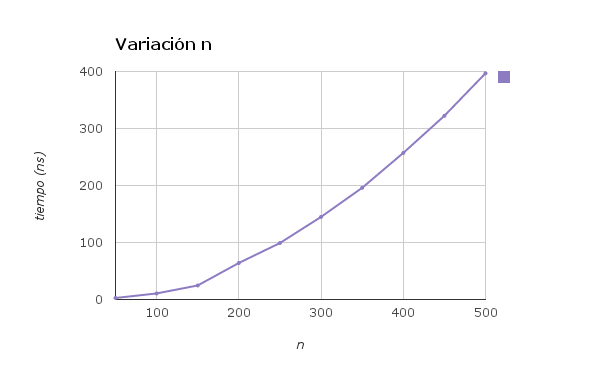
\includegraphics[scale=0.50]{n.png}
	\end{center}
\end{figure}	

En el segundo gráfico, realizamos para cada punto la división del tiempo sobre n. Como estimamos que la curva del gráfico anterior era cuadrática, esta debería ser lineal. Por el gráfico, podemos observar que sigue la tendencia esperada.

\begin{figure}[h]
	\begin{center}
	   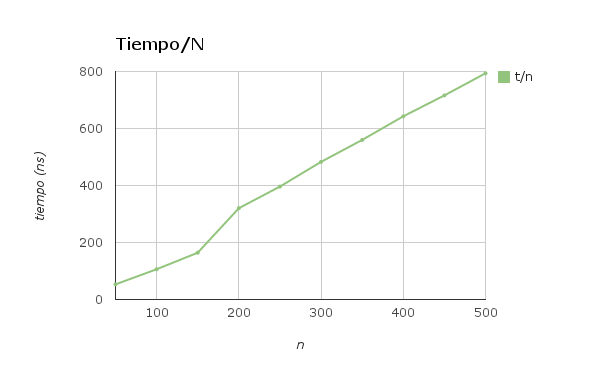
\includegraphics[scale=0.50]{n_sobren.png}
	\end{center}
\end{figure}

Por último, en el tercer gráfico, realizamos la división de cada punto por el tiempo sobre $n^2$. Como esperábamos, la función resultante es constante.

\begin{figure}[h]
	\begin{center}
	   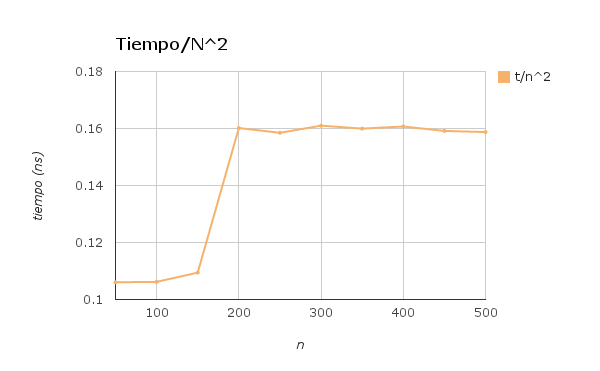
\includegraphics[scale=0.50]{n_sobren2.png}
	\end{center}
\end{figure}

\newpage
\subsubsection{Experimentación variando la cantidad de nodos}

Para este set de experimentos, variamos k (la cantidad de particiones) de 10 a 150 (incrementando de k de a 10) y mantuvimos constante la cantidad de nodos y aristas. Fijamos los nodos en 100 y las aristas en 150.
A partir de los resultados obtenidos, observamos a que el gráfico resultante se condice con la complejidad calculada teóricamente, siendo la variación en k lineal.\\
A continuación, mostraremos la tabla con los valores obtenidos, y los gráficos representando los tiempos de ejecución y la estimación de la complejidad del algoritmo.

\begin{center}
	\begin{tabular}{| l | l | l |}
	\hline
	k & tiempo & $tiempo/k$ \\ \hline
	10 & 2,342375 & 0,2342375\\
	20 & 2,426375 & 0,12131875\\
	30 & 2,508025 & 0,08360083333\\
	40	& 2,552925 & 0,063823125 \\
	50 & 2,674425 & 0,0534885 \\
	60 & 2,71455 & 0,0452425\\
	70 & 2,8401 & 0,04057285714\\
	80 & 2,861375 & 0,0357671875\\
	90 & 2,94165 & 0,032685\\
	100	& 2,968175 & 0,02968175\\
	110	& 3,029625 & 0,02754204545\\
	120	& 3,112725 & 0,025939375\\
	130	& 3,1983 & 0,02460230769\\
	140	& 3,272575 & 0,02337553571\\
	150	& 3,31775 & 0,02211833333\\
	\hline
	\end{tabular}

En el primer gráfico, vemos como la variación del tiempo a medida que se incrementa el número de particiones es lineal en k.

\begin{figure}[h]
	\begin{center}
	   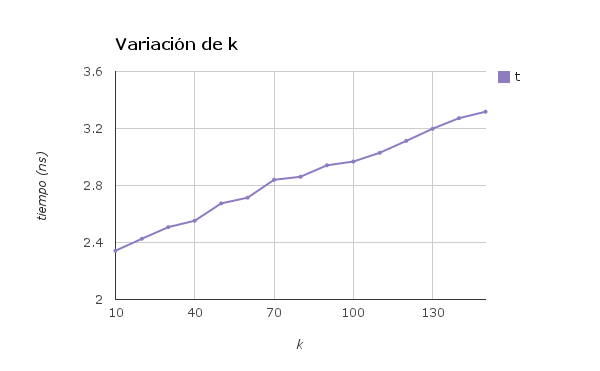
\includegraphics[scale=0.50]{k.png}
	\end{center}
\end{figure}

En este segundo gráfico, podemos corroborarlo, ya que al dividir cada punto por k, obtenemos una gráfica constante.

\begin{figure}[h]
	\begin{center}
	   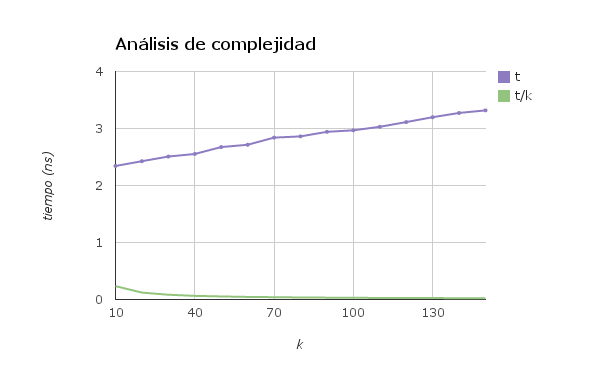
\includegraphics[scale=0.50]{k_sobrek.png}
	\end{center}
\end{figure}

\end{center}

Aunque estos experimentos no bastan para mostrar la correctitud de la demostración de complejidad realizada previamente, los resultados obtenidos parecen indicar que nuestras estimaciones teóricas eran correctas y la complejidad del algoritmo constructivo goloso es $O(k*n^2)$

\end{document}